\documentclass[12pt]{article}
\usepackage[utf8]{inputenc}
\usepackage{amsmath, amssymb}
\usepackage{geometry}
\usepackage{tikz}
\usepackage{pgfplots}
\usepackage{xcolor}
\usepackage{adjustbox}
\usepackage{caption}

\geometry{a4paper, margin=1in}
\pgfplotsset{compat=1.18}

% --- Colors ---
\definecolor{DeepNavy}{HTML}{2E4057}
\definecolor{Teal}{HTML}{048A81}
\definecolor{WarmOrange}{HTML}{E85D04}
\definecolor{Gold}{HTML}{D4A03A}
\definecolor{DeepRed}{HTML}{D62828}
\definecolor{LightGray}{HTML}{F0F0F0}

\usetikzlibrary{shapes.geometric, arrows.meta, positioning, calc, backgrounds, decorations.pathreplacing}

\title{\bfseries Appendix}
\author{Intuition and Derivations}
\date{\today}

\begin{document}

\maketitle

\tableofcontents
\newpage


%%%%%%%%%%%%%%%%%%%%%%%%%%%%%%%%%%%%%%%%%%%%%%%%%%%%%%%%%%%%%%%%%%%%%%%%%%%%%%%%
% Visual Guide
\section{Visual Guide}
\subsection{The Anatomy of a Firm Shock}
For a visual learner, the demand equation $y_{it} = \phi^d p_t + \eta_t + u_{it}$ is a hierarchy of influences.

\begin{center}
    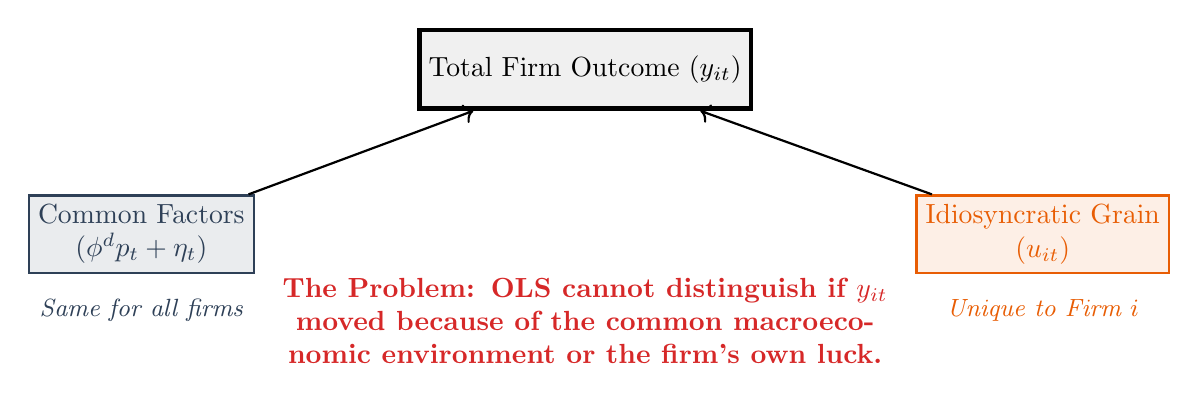
\begin{tikzpicture}[node distance=1.5cm, align=center]
        % Components
        \node (total) [draw, ultra thick, minimum width=4cm, minimum height=1cm, fill=LightGray] {Total Firm Outcome ($y_{it}$)};

        \node (common) [draw, DeepNavy, thick, below left=of total, xshift=-1cm, fill=DeepNavy!10] {Common Factors\\($\phi^d p_t + \eta_t$)};
        \node (idiosyncratic) [draw, WarmOrange, thick, below right=of total, xshift=1cm, fill=WarmOrange!10] {Idiosyncratic Grain\\($u_{it}$)};

        \draw[->, thick] (common) -- (total);
        \draw[->, thick] (idiosyncratic) -- (total);

        % The "Signal" vs "Noise"
        \node[below=0.2cm of common, font=\small\itshape, text=DeepNavy] {Same for all firms};
        \node[below=0.2cm of idiosyncratic, font=\small\itshape, text=WarmOrange] {Unique to Firm $i$};

        % The Problem
        \node[below=2cm of total, text=DeepRed, font=\bfseries, text width=10cm] {The Problem: OLS cannot distinguish if $y_{it}$ moved because of the common macroeconomic environment or the firm's own luck.};
    \end{tikzpicture}
\end{center}

\subsection{The "Differencing" Mechanism}
The GIV ($z_t = y_{St} - y_{Et}$) acts as a filter. Imagine two ``containers'' of shocks. One is size-weighted (dominated by giants) and the other is equally-weighted (the crowd).

\begin{center}
    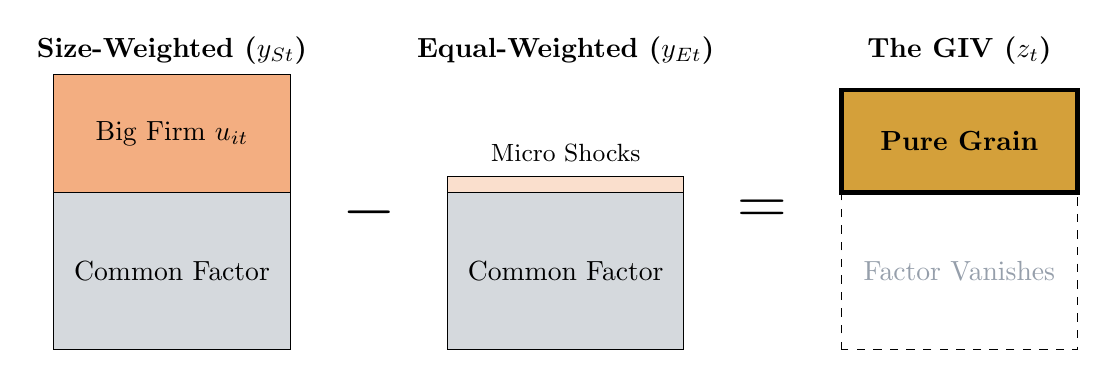
\begin{tikzpicture}
        % Size Weighted
        \begin{scope}[shift={(0,0)}]
            \node[above] at (1.5, 3.5) {\bfseries Size-Weighted ($y_{St}$)};
            \draw[fill=DeepNavy!20] (0,0) rectangle (3,2); % Common
            \draw[fill=WarmOrange!50] (0,2) rectangle (3,3.5); % Big firm shock
            \node at (1.5, 1) {Common Factor};
            \node at (1.5, 2.75) {Big Firm $u_{it}$};
        \end{scope}

        \node at (4, 1.75) {\Huge $-$};

        % Equal Weighted
        \begin{scope}[shift={(5,0)}]
            \node[above] at (1.5, 3.5) {\bfseries Equal-Weighted ($y_{Et}$)};
            \draw[fill=DeepNavy!20] (0,0) rectangle (3,2); % Common
            \draw[fill=WarmOrange!20] (0,2) rectangle (3,2.2); % Average tiny shocks
            \node at (1.5, 1) {Common Factor};
            \node at (1.5, 2.5) {\small Micro Shocks};
        \end{scope}

        \node at (9, 1.75) {\Huge $=$};

        % The GIV
        \begin{scope}[shift={(10,0)}]
            \node[above] at (1.5, 3.5) {\bfseries The GIV ($z_t$)};
            \draw[dashed] (0,0) rectangle (3,2); % Vanished common
            \draw[fill=Gold, ultra thick] (0,2) rectangle (3,3.3); % Pure grain
            \node[text=DeepNavy!50] at (1.5, 1) {Factor Vanishes};
            \node at (1.5, 2.65) {\bfseries Pure Grain};
        \end{scope}
    \end{tikzpicture}
\end{center}

\newpage

\subsection{Why Granularity Matters (The Power Law)}
GIV only works if the "Big Firm Shock" in the previous diagram is large enough to survive the averaging. In a "Normal" economy (left), the GIV is just noise. In a "Granular" economy (right), the giants move the needle.

\begin{center}
    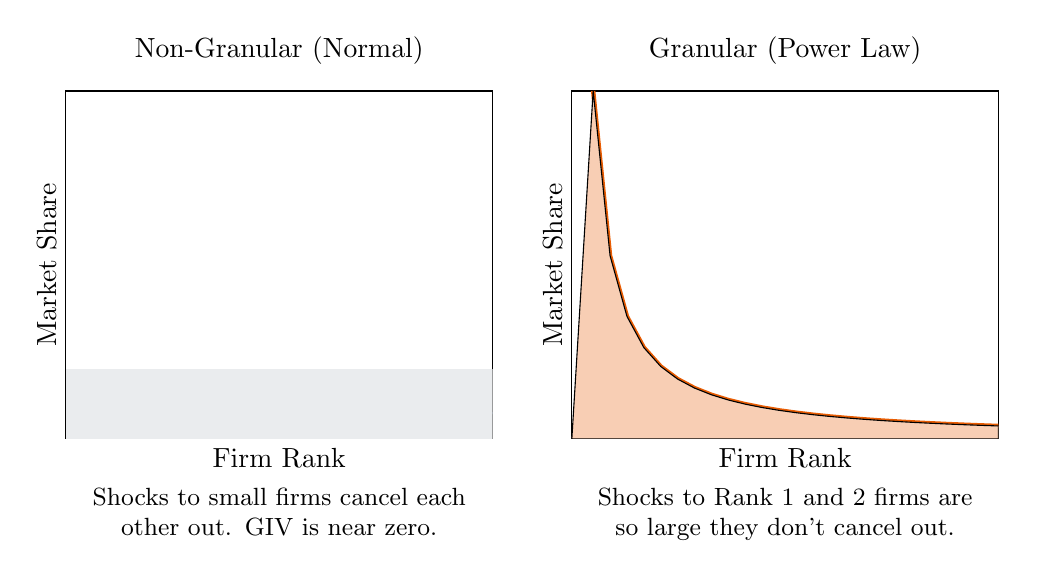
\begin{tikzpicture}
        \begin{axis}[
                name=normal,
                width=7cm, height=6cm,
                title={Non-Granular (Normal)},
                xlabel={Firm Rank}, ylabel={Market Share},
                xmin=0, xmax=20, ymin=0, ymax=1,
                ticks=none
            ]
            \addplot[DeepNavy, thick, domain=1:20] {0.2 * exp(-0.05*x)};
            \fill[DeepNavy!10] (axis cs:0,0) rectangle (axis cs:20,0.2);
        \end{axis}

        \begin{axis}[
                name=granular,
                at={($(normal.right of south east)+(1cm,0)$)},
                anchor=south west,
                width=7cm, height=6cm,
                title={Granular (Power Law)},
                xlabel={Firm Rank}, ylabel={Market Share},
                xmin=0, xmax=20, ymin=0, ymax=1,
                ticks=none
            ]
            \addplot[WarmOrange, ultra thick, domain=1:20] {1/x^1.1};
            \draw[fill=WarmOrange!30] (axis cs:0,0) -- plot[domain=1:20] (axis cs:\x,{1/\x^1.1}) -- (axis cs:20,0) -- cycle;
        \end{axis}

        \node[below=0.5cm of normal, text width=6cm, align=center, font=\small] {Shocks to small firms cancel each other out. GIV is near zero.};
        \node[below=0.5cm of granular, text width=6cm, align=center, font=\small] {Shocks to Rank 1 and 2 firms are so large they don't cancel out.};
    \end{tikzpicture}
\end{center}

\subsection{Conceptual Flow of Identification}
How does $z_t$ help us find the causal effect $\psi$?

\begin{center}
    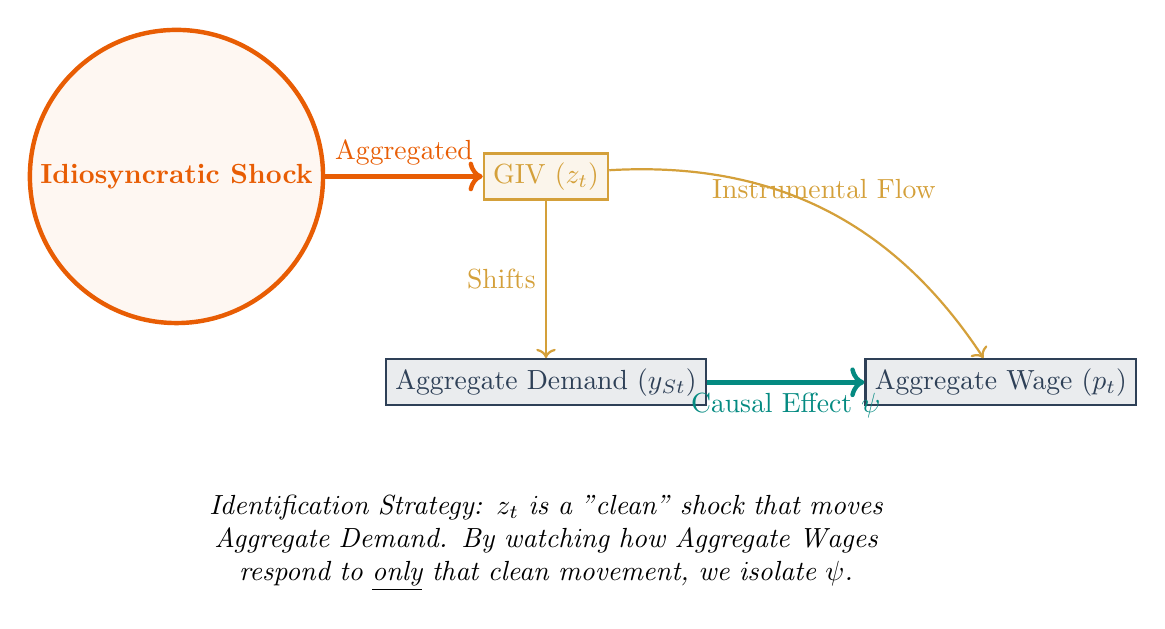
\begin{tikzpicture}[node distance=2cm, auto]
        \node (shock) [circle, draw, WarmOrange, ultra thick, fill=WarmOrange!5] {\bfseries Idiosyncratic Shock};
        \node (giv) [rectangle, draw, Gold, thick, right=of shock, fill=Gold!10] {GIV ($z_t$)};
        \node (aggregate) [rectangle, draw, DeepNavy, thick, below=of giv, fill=DeepNavy!10] {Aggregate Demand ($y_{St}$)};
        \node (price) [rectangle, draw, DeepNavy, thick, right=of aggregate, fill=DeepNavy!10] {Aggregate Wage ($p_t$)};

        \draw[->, ultra thick, WarmOrange] (shock) -- (giv) node[midway, above] {Aggregated};
        \draw[->, thick, Gold] (giv) -- (aggregate) node[midway, left] {Shifts};
        \draw[->, thick, Gold] (giv) to [bend left] node[above] {Instrumental Flow} (price);

        \draw[->, ultra thick, Teal] (aggregate) -- (price) node[midway, below] {Causal Effect $\psi$};

        \node[below=1cm of aggregate, text width=12cm, align=center, font=\itshape] {Identification Strategy: $z_t$ is a "clean" shock that moves Aggregate Demand. By watching how Aggregate Wages respond to \underline{only} that clean movement, we isolate $\psi$.};
    \end{tikzpicture}
\end{center}
%%%%%%%%%%%%%%%%%%%%%%%%%%%%%%%%%%%%%%%%%%%%%%%%%%%%%%%%%%%%%%%%%%%%%%%%%%%%%%%%
% Derivation of equation 41
\section{Derivation of equation 41}
\subsection{The Base Model}
We start with the demand equation for firm $i$ at time $t$, as given by Equation 39:
\begin{equation}
    y_{it} = \phi^d p_t + \eta_t + u_{it} \tag{39}
\end{equation}
where:
\begin{itemize}
    \item $y_{it}$ is the outcome for firm $i$.
    \item $p_t$ is the common price (or wage).
    \item $\phi^d$ is the demand elasticity.
    \item $\eta_t$ is a common aggregate shock.
    \item $u_{it}$ is the idiosyncratic shock to firm $i$.
\end{itemize}

\subsection{Deriving the Size-Weighted Aggregate ($y_{St}$)}
The size-weighted outcome is defined as $y_{St} = \sum_{i=1}^N S_i y_{it}$, where $S_i$ are weights such that $\sum S_i = 1$.

Substituting Equation 39 into this definition:
\begin{align*}
    y_{St} & = \sum_{i=1}^N S_i (\phi^d p_t + \eta_t + u_{it})                                 \\
    y_{St} & = \sum_{i=1}^N S_i \phi^d p_t + \sum_{i=1}^N S_i \eta_t + \sum_{i=1}^N S_i u_{it}
\end{align*}

Since $\phi^d$, $p_t$, and $\eta_t$ do not depend on the index $i$, we can pull them out of the summations:
\begin{align*}
    y_{St} & = \phi^d p_t \left( \sum_{i=1}^N S_i \right) + \eta_t \left( \sum_{i=1}^N S_i \right) + \sum_{i=1}^N S_i u_{it}
\end{align*}

Using the property $\sum S_i = 1$ and defining the size-weighted idiosyncratic shock as $u_{St} = \sum S_i u_{it}$, we get:
\begin{equation}
    y_{St} = \phi^d p_t + \eta_t + u_{St}
\end{equation}

\subsection{Deriving the Equal-Weighted Aggregate ($y_{Et}$)}
The equal-weighted outcome is defined as $y_{Et} = \frac{1}{N} \sum_{i=1}^N y_{it}$.

Substituting Equation 39:
\begin{align*}
    y_{Et} & = \frac{1}{N} \sum_{i=1}^N (\phi^d p_t + \eta_t + u_{it})                                                 \\
    y_{Et} & = \frac{1}{N} \sum_{i=1}^N \phi^d p_t + \frac{1}{N} \sum_{i=1}^N \eta_t + \frac{1}{N} \sum_{i=1}^N u_{it}
\end{align*}

Again, pulling constants out of the summations:
\begin{align*}
    y_{Et} & = \phi^d p_t \left( \frac{1}{N} \sum_{i=1}^N 1 \right) + \eta_t \left( \frac{1}{N} \sum_{i=1}^N 1 \right) + \frac{1}{N} \sum_{i=1}^N u_{it}
\end{align*}

Since $\frac{1}{N} \sum_{i=1}^N 1 = \frac{1}{N} \cdot N = 1$, and defining the equal-weighted idiosyncratic shock as $u_{Et} = \frac{1}{N} \sum u_{it}$, we get:
\begin{equation}
    y_{Et} = \phi^d p_t + \eta_t + u_{Et}
\end{equation}

\subsection{Result (Equation 41)}
Combining these two results, we obtain Equation 41:
\begin{align}
    y_{St} & = \phi^d p_t + \eta_t + u_{St} \notag   \\
    y_{Et} & = \phi^d p_t + \eta_t + u_{Et} \tag{41}
\end{align}


%%%%%%%%%%%%%%%%%%%%%%%%%%%%%%%%%%%%%%%%%%%%%%%%%%%%%%%%%%%%%%%%%%%%%%%%%%%%%%%%
% Derivation of equation on slide 9
\section{Derivation of equation on slide 9}
\subsection{Introduction}
Slide 9 of the presentation demonstrates how the Granular Instrumental Variable ($z_t$) can be used to identify both the supply elasticity ($\psi$) and the demand elasticity ($\phi^d$). This document provides the underlying derivations and the statistical assumptions required for these results.

\subsection{The Core Model and the GIV}
Recall the system of equations from slide 5:
\begin{align}
    p_t    & = \psi y_{St} + \epsilon_t \label{eq:supply} \tag{38}          \\
    y_{it} & = \phi^d p_t + \eta_t + u_{it} \label{eq:demand_firm} \tag{39}
\end{align}
where $y_{St} = \sum S_i y_{it}$ is the size-weighted aggregate outcome. From slide 8, we define the Granular Instrumental Variable ($z_t$) as the difference between size-weighted and equal-weighted aggregate outcomes:
\begin{equation}
    z_t = y_{St} - y_{Et} = u_{St} - u_{Et} \label{eq:giv_def} \tag{42}
\end{equation}
where $u_{St} = \sum S_i u_{it}$ and $u_{Et} = \frac{1}{N} \sum u_{it}$.

\subsection{The Exogeneity Condition}
The fundamental assumption of the GIV approach is that the idiosyncratic shocks $u_{it}$ are independent of the aggregate shocks $\epsilon_t$ and $\eta_t$. Since $z_t$ is a linear combination of only idiosyncratic shocks, it follows that:
\begin{equation}
    \mathbb{E}[z_t \epsilon_t] = 0 \quad \text{and} \quad \mathbb{E}[z_t \eta_t] = 0 \label{eq:exogeneity}
\end{equation}
This exogeneity allows $z_t$ to serve as a valid instrument.

\subsection{Identifying Supply Elasticity ($\psi$)}
To find $\psi$, we use $z_t$ as an instrument for $y_{St}$ in the supply equation (\ref{eq:supply}). We take the expectation of the product of the supply equation and the instrument:
\begin{align*}
    \mathbb{E}[p_t z_t] & = \mathbb{E}[(\psi y_{St} + \epsilon_t) z_t]               \\
    \mathbb{E}[p_t z_t] & = \psi \mathbb{E}[y_{St} z_t] + \mathbb{E}[\epsilon_t z_t]
\end{align*}
By the exogeneity condition in (\ref{eq:exogeneity}), $\mathbb{E}[\epsilon_t z_t] = 0$. Thus:
\begin{equation}
    \psi = \frac{\mathbb{E}[p_t z_t]}{\mathbb{E}[y_{St} z_t]}
\end{equation}
This is the standard IV formula where $z_t$ instruments for $y_{St}$.

\subsection{Identifying Demand Elasticity ($\phi^d$)}
To find $\phi^d$, we use the equal-weighted aggregate demand equation derived on slide 8:
\begin{equation}
    y_{Et} = \phi^d p_t + \eta_t + u_{Et} \tag{41}
\end{equation}
We aim to show that $\mathbb{E}[(y_{Et} - \phi^d p_t) z_t] = 0$. Substituting the demand equation:
\begin{equation}
    \mathbb{E}[(y_{Et} - \phi^d p_t) z_t] = \mathbb{E}[(\eta_t + u_{Et}) z_t] = \mathbb{E}[\eta_t z_t] + \mathbb{E}[u_{Et} z_t]
\end{equation}
We already know $\mathbb{E}[\eta_t z_t] = 0$. Now we examine $\mathbb{E}[u_{Et} z_t]$. Under the assumption that $u_{it}$ are i.i.d. with variance $\sigma_u^2$:
\begin{align*}
    \mathbb{E}[u_{Et} z_t] & = \mathbb{E}[u_{Et} (u_{St} - u_{Et})]                                                                                                                                             \\
                           & = \mathbb{E}[u_{Et} u_{St}] - \mathbb{E}[u_{Et}^2]                                                                                                                                 \\
                           & = \mathbb{E} \left[ \left( \frac{1}{N} \sum_{i} u_{it} \right) \left( \sum_{j} S_j u_{jt} \right) \right] - \mathbb{E} \left[ \left( \frac{1}{N} \sum_{i} u_{it} \right)^2 \right] \\
                           & = \frac{1}{N} \sum_{i} S_i \sigma_u^2 - \frac{1}{N^2} \sum_{i} \sigma_u^2                                                                                                          \\
                           & = \frac{1}{N} \sigma_u^2 (1) - \frac{1}{N} \sigma_u^2 = 0
\end{align*}
Since $\mathbb{E}[u_{Et} z_t] = 0$, it follows that $\mathbb{E}[(y_{Et} - \phi^d p_t) z_t] = 0$. Rearranging:
\begin{align*}
    \mathbb{E}[y_{Et} z_t] & = \phi^d \mathbb{E}[p_t z_t]                         \\
    \phi^d                 & = \frac{\mathbb{E}[y_{Et} z_t]}{\mathbb{E}[p_t z_t]}
\end{align*}
This identifies the demand elasticity using the same granular instrument $z_t$.

%%%%%%%%%%%%%%%%%%%%%%%%%%%%%%%%%%%%%%%%%%%%%%%%%%%%%%%%%%%%%%%%%%%%%%%%%%%%%%%%
% Full model deep dive

\section{Full model deep dive}

\subsection{Introduction}
Slides 11 and 12 move from the "Simple Model" (where every firm responds identically to the macroeconomy) to the "Full Model." This is crucial because, in reality, superstar firms often have different sensitivities to interest rates, exchange rates, or global demand than small firms.

\subsection{Slide 11: The Full Factor Model}

\subsection{The Equation}
We start with the demand equation for firm $i$:
\begin{equation}
    y_{it} = \phi p_t + \lambda_i \eta_t + u_{it} \label{eq:full}
\end{equation}
where $\lambda_i$ is the \textbf{factor loading}.

\subsection{Intuition: What is a Factor Loading?}
A factor loading $\lambda_i$ measures firm $i$'s \textit{sensitivity} to a common macro shock $\eta_t$.
\begin{itemize}
    \item \textbf{Example:} If $\eta_t$ is a surge in energy prices, an airline like Delta might have a high $\lambda_i$ (very sensitive), while a software firm like Microsoft might have a low $\lambda_i$.
    \item \textbf{Heterogeneity:} In the simple model, we assumed $\lambda_i = 1$ for everyone. In the full model, we acknowledge that large firms might be more (or less) sensitive to macro trends than the average firm.
\end{itemize}

\subsection{Derivation: Why the Simple GIV Fails}
The simple GIV is defined as $z_t^{simple} = y_{St} - y_{Et}$. Let's derive its components using Equation \ref{eq:full}:

1. \textbf{Size-weighted average ($y_{St}$):}
\begin{align*}
    y_{St} & = \sum S_i y_{it} = \sum S_i (\phi p_t + \lambda_i \eta_t + u_{it})                                                               \\
           & = \phi p_t \underbrace{\sum S_i}_{1} + \eta_t \underbrace{\sum S_i \lambda_i}_{\lambda_S} + \underbrace{\sum S_i u_{it}}_{u_{St}} \\
           & = \phi p_t + \lambda_S \eta_t + u_{St}
\end{align*}

2. \textbf{Equal-weighted average ($y_{Et}$):}
\begin{align*}
    y_{Et} & = \frac{1}{N} \sum y_{it} = \phi p_t + \eta_t \underbrace{\frac{1}{N} \sum \lambda_i}_{\lambda_E} + u_{Et} \\
           & = \phi p_t + \lambda_E \eta_t + u_{Et}
\end{align*}

3. \textbf{The Resulting GIV:}
\begin{equation}
    z_t^{simple} = y_{St} - y_{Et} = \mathbf{(\lambda_S - \lambda_E) \eta_t} + (u_{St} - u_{Et})
\end{equation}

\textbf{The Problem:} If large firms have different macro-sensitivities than small firms ($\lambda_S \neq \lambda_E$), then the instrument $z_t^{simple}$ is correlated with the common shock $\eta_t$. It is no longer a "pure" idiosyncratic shock; it is "leaky."

\subsection{Slide 12: The Solution (Optimal Weights)}

\subsection{The Goal: Orthogonality}
We want to choose a new set of weights, $\Gamma_i$, to construct a valid GIV: $z_t = \sum \Gamma_i y_{it}$. For this to be a valid instrument for the supply equation, it must be uncorrelated with the macro shock $\eta_t$.

\subsection{Derivation of the Orthogonality Condition}
Substitute Equation \ref{eq:full} into the definition of the weighted GIV:
\begin{align*}
    z_t & = \sum \Gamma_i (\phi p_t + \lambda_i \eta_t + u_{it})                               \\
        & = \phi p_t (\sum \Gamma_i) + \eta_t (\sum \Gamma_i \lambda_i) + \sum \Gamma_i u_{it}
\end{align*}
To ensure $z_t$ contains \textit{only} idiosyncratic shocks ($u_{it}$), we must satisfy two conditions:
\begin{enumerate}
    \item $\sum \Gamma_i = 0$: This removes the endogenous price $p_t$.
    \item $\sum \Gamma_i \lambda_i = 0$: This removes the common macro shock $\eta_t$.
\end{enumerate}

\subsection{Why not just Firm Size ($S_i$)?}
\begin{itemize}
    \item \textbf{Power vs. Validity:} Firm size ($S_i$) gives the instrument its \textbf{power}. We want the instrument to be large, and only large firms can create aggregate "granular" ripples.
    \item \textbf{The Conflict:} If we use $z_t = \sum (S_i - 1/N) y_{it}$, we have power, but we lack validity if $S_i$ is correlated with $\lambda_i$ (e.g., if big firms are more sensitive to macro shocks).
    \item \textbf{The "Tilt":} We start with firm sizes $S_i$ but then "tilt" or project them until they are perpendicular (orthogonal) to the macro-sensitivities $\lambda_i$.
\end{itemize}

\subsection{Mathematical Solution (Projection)}
In matrix form, we want $\Gamma$ to be as close as possible to $S$ but satisfy $\Gamma \perp \lambda$. This is a standard projection problem:
\begin{equation}
    \Gamma = S - \lambda (\lambda' \lambda)^{-1} \lambda' S
\end{equation}
\textbf{Intuition:} We take the firm sizes and subtract the portion of size that is explained by macro-sensitivity. What remains is "Pure Granular Weight."

\subsection{Summary}
\begin{itemize}
    \item \textbf{Factor Loadings ($\lambda_i$)}: Firm-specific sensitivities to the macroeconomy.
    \item \textbf{Validity}: We cannot use raw size if size correlates with macro-sensitivity.
    \item \textbf{Optimal Weights ($\Gamma_i$)}: The "tilted" versions of size weights that satisfy $\sum \Gamma_i \lambda_i = 0$.
\end{itemize}

%%%%%%%%%%%%%%%%%%%%%%%%%%%%%%%%%%%%%%%%%%%%%%%%%%%%%%%%%%%%%%%%%%%%%%%%%%%%%%%%
% Gamma intuition

\section{Gamma intuition}


\subsection{Recap: The Simple vs. The Full Model}
In the simple model, we assume all firms respond identically to macro shocks. The GIV was simply:
\begin{equation}
    z_t^{simple} = \sum (S_i - 1/N) y_{it}
\end{equation}
This works because $S_i - 1/N$ is orthogonal to a constant factor (where every firm has $\lambda_i = 1$). However, when firms have heterogeneous sensitivities $\lambda_i$, the simple weights fail. We need $\Gamma$.

\subsection{Intuition: $\Gamma$ as "De-biased" Firm Size}

\subsection{The Simple GIV as a Special Case}
Think of the simple GIV weights as $\Gamma_i^{simple} = S_i - \bar{S}$. We take the raw size and subtract the mean size. This "centers" the weights around zero, which kills any factor that hits everyone equally.

\subsection{The Problem with Raw Size}
If large firms are systematically more sensitive to interest rates (a common factor $\eta_t$), then the size-weighted outcome $y_{St}$ will move whenever interest rates move. If we use $y_{St}$ as an instrument, we are accidentally instrumenting with interest rate shocks, not idiosyncratic firm shocks.

\subsection{The Logic of $\Gamma$}
$\Gamma$ is the part of firm size that is \textbf{unrelated} to macro-sensitivity.
\begin{itemize}
    \item We ask: "How much of this firm's size is explained by its factor loading $\lambda_i$?"
    \item We subtract that "explained" part from the actual size.
    \item The result, $\Gamma_i$, is the "Pure Granular Weight."
\end{itemize}
If $\lambda_i$ is completely uncorrelated with $S_i$, then $\Gamma$ will look almost exactly like the simple GIV weights. If they are correlated, $\Gamma$ "tilts" the weights to protect the instrument's validity.

\subsection{The Math: $\Gamma$ as a Projection Residual}

Mathematically, we want to find weights $\Gamma$ that are as close as possible to the size weights $S$ (for power), but are orthogonal to the loadings $\lambda$ (for validity).

We solve the following optimization problem:
\begin{equation}
    \min_{\Gamma} \sum_{i=1}^N (\Gamma_i - S_i)^2 \quad \text{subject to} \quad \sum \Gamma_i = 0, \quad \sum \Gamma_i \lambda_i = 0
\end{equation}

The solution to this problem is equivalent to the **residual** of a linear regression. If we regress the vector of sizes $S$ on a constant and the vector of loadings $\lambda$:
\begin{equation}
    S_i = \alpha + \beta \lambda_i + \text{residual}_i
\end{equation}
Then the optimal weight $\Gamma_i$ is exactly that residual.

\subsection{General Matrix Formula}
If there are multiple factors (a matrix $\Lambda$), the formula is:
\begin{equation}
    \Gamma = M_{\tilde{\Lambda}} S = (I - \tilde{\Lambda} (\tilde{\Lambda}' \tilde{\Lambda})^{-1} \tilde{\Lambda}') S
\end{equation}
where $\tilde{\Lambda} = [\mathbf{1}, \Lambda]$ is the matrix of loadings plus a constant. $M_{\tilde{\Lambda}}$ is the "annihilator matrix" that projects $S$ into the space orthogonal to the factors.


\subsection{Summary}
The transition from $z^{simple}$ to $z^{\Gamma}$ is a move from **demeaning** to **orthogonalizing**. In the simple model, we demean by subtracting $1/N$. In the full model, we orthogonalize by subtracting the projection of size onto macro-loadings.


%%%%%%%%%%%%%%%%%%%%%%%%%%%%%%%%%%%%%%%%%%%%%%%%%%%%%%%%%%%%%%%%%%%%%%%%%%%%%%%%
% Derivation of equation on slide 9
% Gamma derivation
\section{Derivation of Gamma}

\subsection{The Optimization Problem}
The goal of finding optimal GIV weights $\Gamma$ is to stay as close as possible to the power-maximizing size weights $S$, while ensuring orthogonality to common factors (captured by loadings $\Lambda$) and a constant (to ensure the weights sum to zero).

Mathematically, we solve:
\begin{equation}
    \min_{\Gamma} \frac{1}{2} \sum_{i=1}^N (\Gamma_i - S_i)^2
\end{equation}
subject to:
\begin{align}
    \sum_{i=1}^N \Gamma_i           & = 0 \tag{Constraint 1: Sum to Zero}                \\
    \sum_{i=1}^N \Gamma_i \lambda_i & = 0 \tag{Constraint 2: Orthogonality to $\lambda$}
\end{align}

\subsection{Lagrangian Setup}
We define the Lagrangian $\mathcal{L}$ with multipliers $\mu_1$ and $\mu_2$:
\begin{equation}
    \mathcal{L}(\Gamma, \mu_1, \mu_2) = \frac{1}{2} \sum_{i=1}^N (\Gamma_i - S_i)^2 + \mu_1 \left( \sum_{i=1}^N \Gamma_i \right) + \mu_2 \left( \sum_{i=1}^N \Gamma_i \lambda_i \right)
\end{equation}

\subsection{First Order Conditions (FOCs)}
Differentiating with respect to the decision variable $\Gamma_i$:
\begin{equation}
    \frac{\partial \mathcal{L}}{\partial \Gamma_i} = (\Gamma_i - S_i) + \mu_1 + \mu_2 \lambda_i = 0
\end{equation}
Rearranging for $\Gamma_i$, we get the structure of the solution:
\begin{equation} \label{eq:gamma_sol}
    \Gamma_i = S_i - (\mu_1 + \mu_2 \lambda_i)
\end{equation}

\subsection{Equivalence to Linear Regression}
Recall the standard OLS model where we regress $S_i$ on a constant and $\lambda_i$:
\begin{equation}
    S_i = \alpha + \beta \lambda_i + \epsilon_i
\end{equation}
The OLS estimator $(\hat{\alpha}, \hat{\beta})$ minimizes the sum of squared residuals $\sum \epsilon_i^2$. The resulting residuals are defined as:
\begin{equation}
    \hat{\epsilon}_i = S_i - (\hat{\alpha} + \hat{\beta} \lambda_i)
\end{equation}
Comparing this to Equation \ref{eq:gamma_sol}, we see that $\Gamma_i$ has the exact same functional form as the OLS residual $\hat{\epsilon}_i$, where the Lagrange multipliers $\mu_1$ and $\mu_2$ play the roles of the OLS coefficients $\hat{\alpha}$ and $\hat{\beta}$.

\subsection{Why the Constraints Matter}
The "Normal Equations" that solve OLS are:
\begin{enumerate}
    \item $\sum \hat{\epsilon}_i = 0$ (The sum of residuals is zero if an intercept is included).
    \item $\sum \hat{\epsilon}_i \lambda_i = 0$ (Residuals are orthogonal to the regressors).
\end{enumerate}
These are exactly our two constraints! Therefore, the values of $\mu_1$ and $\mu_2$ that satisfy our constraints are precisely the OLS coefficients $\hat{\alpha}$ and $\hat{\beta}$.

\subsection{Conclusion}
Solving for the optimal weights $\Gamma$ is equivalent to regressing the vector of sizes $S$ on the factor loadings (and a constant) and taking the residuals.
\begin{equation}
    \Gamma = \text{Residuals of } (S \sim 1 + \Lambda)
\end{equation}
In matrix notation, this is the projection:
\begin{equation}
    \Gamma = M_X S = (I - X(X'X)^{-1}X')S
\end{equation}
where $X = [\mathbf{1}, \Lambda]$. This projection removes the "macro-contaminated" portion of the firm size, leaving only the idiosyncratic granular component.



\end{document}
